Se connecter sur ChromaCase avec Google vous permet de retrouver vos progrès et historique d’une session précédente, en utilisant votre compte Google.

À partir de la page d’accueil, il faut cliquer sur le bouton \textit{Authenticate}.

\begin{figure}[H]
	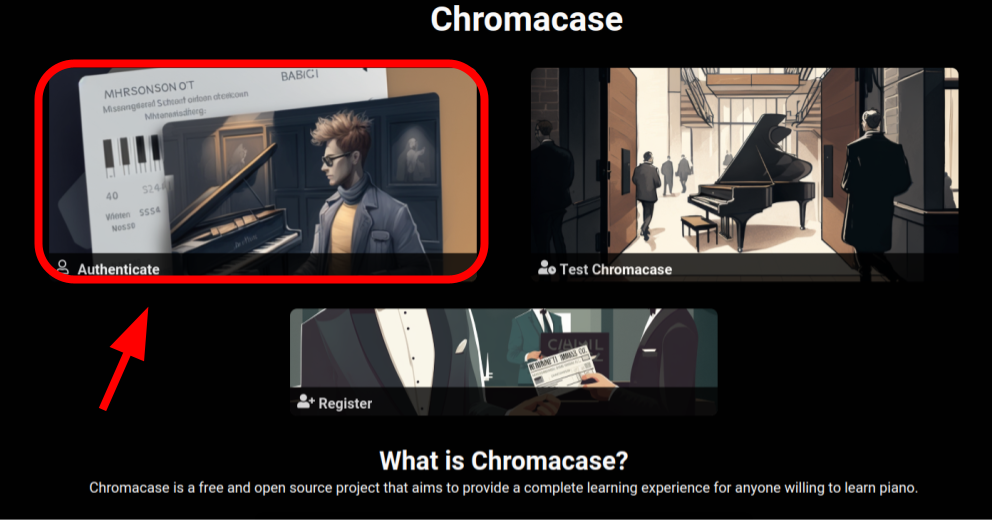
\includegraphics[width=\linewidth]{../\dir/guide/auth/authenticate.png}
	\caption{Accéder à la page d'authentification}
\end{figure}

Une fois rendu sur le formulaire, cliquez sur le bouton \textit{Continue With Google}.

\begin{figure}[H]
	\begin{center}
		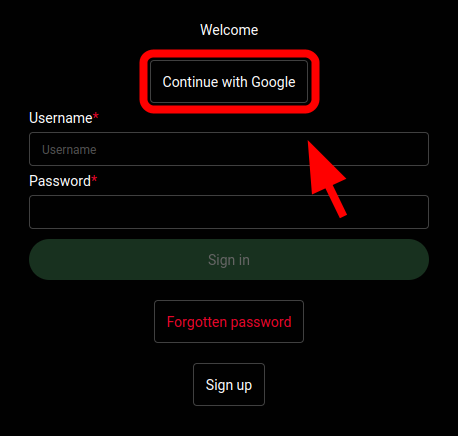
\includegraphics[width=0.5\linewidth]{../\dir/guide/auth/signin-google.png}
		\caption{Se connecter avec Google}
	\end{center}
\end{figure}

Vous serez redirigé vers un formulaire de connexion Google. Une fois rempli et validé, vous serez redirigé.e sur votre page personnelle.